%!TEX TS-program = pdflatex
%!TEX root = main.tex
%!TEX encoding = UTF-8 Unicode

\section{Signed Distance Functions}
\subsection{Theory}
As Hart says in the introduction of
\emph{``Sphere tracing: a geometric method for antialiased ray tracing of implicit surfaces"}
\cite{hart1996}, an implicit surface is defined by a function that, given a point in space, indicates whether the point is inside, on or outside the surface.
The implicit surface can be defined either with an algebraic distance or with a geometric distance.
As an example, the unit sphere can be defined with the algebraic implicit equation
$$ x^2 + y^2 + z^2 - 1 = 0 $$
or geometrically with
$$ \norm{x} - 1= 0 $$
where $x \in \R^3$ and $\norm{\cdot}$ is the Euclidean magnitude $\sqrt{x^2 + y^2 + z^2}$
.
In this document we will not analyze the differences between the two representations because we will use simple surfaces, for which the equations can be translated easily from one form to the other.
Note that the two equations have the same value, i.e. Zero, when the provided point belong to the surface, and both became negative when the point is inside the surface.
% Formalizing, we can say a \emf{distance surface} is implicitly defined by a function 
\begin{definition}[Distance Surface]
  A distance surface is implicitly defined by a function 
$f : \R^3 \to \R$ that characterizes $A \subset \R^3$, set of points that are on or inside the implicit surface:
$$ A = \{ x: f(x) \leq 0\} $$
\end{definition}
\noindent
The surface can be also defined with $f^{-1}(0)$, which gives exactly the points on the surface.
Even if the continuity of $f$ and its negativity on the interior of the surface are not strictly necessary properties, they come useful in practice so, when possible, they are preferable.
We can define the surface from the outside using a \emph{point-to-set} distance:
$$
d(x,A) = min_{y \in A} \norm{x - y}
$$
Thus $d(x,A)$, given a point $x \in \R^3$, returns the shortest distance to the surface defined by $A$.
Note that here we interchange $d(x,A)$ with $d(x, f^{-1}(0))$ even if they are slightly different.
We can do that because usually we'll handle points that aren't in surfaces interiors\footnote{
  In the implementation one must consider this cases e.g. the camera (wrongly) is inside an object
}.
%%We say that $f: \R^3 \to \R$ is a \emph{signed distance bound} of its implicit surface $f^{-1}(0)$ if and only if
%%$$
%%\abs{f(x)} \leq d(x,f^{-1}(0))
%%$$
\begin{definition}[Signed Distance Bound]
We say that $f: \R^3 \to \R$ is a signed distance bound of its implicit surface $f^{-1}(0)$ if and only if
\begin{equation}\label{eq:sdb}
\abs{f(x)} \leq d(x,f^{-1}(0))
\end{equation}
\end{definition}

\noindent
In other words, the definition says that $f$ is always at least as cautious as the true distance function $d(x,f^{-1}(0))$.
This means that we can move $x$ by $d(x,f^{-1}(0))$ in every direction and in the worst case (or best) we'll just hit the surface.
%Using $f$ we'll never get to the interior of the surface.
Moving in this way we'll never put the point at the interior of the surface.
%When in \autoref{eq:sdb} holds the equality, $f$ is a \emph{signed distance function} (SDF) and returns the exact distance to the surface, so moving $x$ by this distance (in the right direction) means putting it exactly on the implicit surface.

\begin{definition}[Signed Distance Function]
We say that $f$ is a signed distance function (SDF) when holds
\begin{equation}\label{eq:sdf}
\abs{f(x)} = d(x,f^{-1}(0))
\end{equation}
\end{definition}

\noindent
An SDF returns the exact distance to the surface, so moving $x$ by this distance (in the right direction) means putting it exactly on the implicit surface $f^{-1}(0)$.
In the introductory article
\emph{``Rendering Implicit Surfaces and Distance Fields: Sphere Tracing"}\cite{scratch_sdf}
by \url{scratchapixel.com},
these concepts are emphasized calling them respectively: 
\emph{distance underestimate (implicit) functions} (DUFs) and 
\emph{distance implicit functions} (DIFs).
Remembering that $DUF(x) \leq DIF(x)$ for every DUFs and DIFs respecting the definitions above.

% TODO Nice imgs?
% https://www.scratchapixel.com/images/upload/distance-fields/sphere-tracing-fig7.png?

For simple shapes we can derive SDFs by hand, but when it's not feasible we can use the Lipschitz constant $\lambda$, as Hart\cite{hart1996} suggested.

\begin{definition}{Lipschitz Function}
We say that a function $f : \R^3 \to \R$ is Lipschitz over a domain $D$ if and only if there is a positive, finite, constant $\lambda$ such that
\begin{equation}\label{eq:lip_fun}
\abs{f(x) - f(y)} \leq \lambda \norm{x - y}
\end{equation}
Such $\lambda$ is called the Lipschitz constant.
\end{definition}
\noindent
Of course there is no upper limit to $\lambda$, but there is a lower bound.
Let $Lip(f)$ be the function returning such minimum value.
Manipulating \autoref{eq:lip_fun} we can observe that
\begin{align*}
  \lambda &\geq \dfrac{\abs{f(x) - f(y)}}{\norm{x - y}} \\
  \lambda &\geq \dfrac{f(x) - f(y)}{\norm{x - y}} \\ %\;\;\; \text{ remember $\lambda$ is positive } \\
  \lambda &\geq \lim_{\norm{x-y} \to 0} \dfrac{f(x) - f(y)}{x - y} = f'(x)
\end{align*}
the last step, given the continuity of $f$, permits us to estimate a safe lower bound for the Lipschitz constant.
To be precise what we have to do is to compute the derivative maximum value, therefore we need to find the solutions to the function second order derivative $f''(x)$.

The following theorem (from \cite{hart1996}) explains why having such a $\lambda$ (or a suitable approximation) is so important: because it gives us a general method for computing a DUF for any Lipschitz function.
\begin{theorem}
  Let $f$ be Lipschitz with Lipschitz constant $\lambda$.
  Then the function $f / \lambda$ is a SDF of its implicit surface.
\end{theorem}
\begin{proof}
  Given a point $x$ and a point $y \in f^{-1}(0)$ such that
  \begin{equation}
  \label{eq:hypot}
    \norm{x - y} = d(x, f^{-1}(0))
  \end{equation}
  Because $f$ is Lipschitz, holds
  $$ \abs{f(x) - f(y)} \leq \lambda \norm{x - y} $$
  and because $y$ is on the surface $f(y) = 0$, so
  \begin{align*}
    \abs{f(x)} &\leq \lambda \norm{x - y} \\
    \abs{f(x)} &\leq \lambda d(x, f^{-1}(0)) \;\;\; \text{by \autoref{eq:hypot}}
  \end{align*}
  Hence
  $ \dfrac{\abs{f(x)}}{\lambda} \leq d(x, f^{-1}(0)) $
  %%$$ \dfrac{\abs{f(x)}}{\lambda} &\leq d(x, f^{-1}(0)) $$
  is a signed distance bound (DUF) for any Lipschitz function $f$.
\end{proof}
One secondary thing to note is that an SDF can return any negative number when the given point is inside the surface.
A common choice is to give a constant negative number i.e. $-1$.

% TODO say or not to say?
%Note that a Lipschitz constant of the sum of two functions results from the sum of the functions' Lipschitz constant, and a Lipschitz constant of the composition of functions results from the product of the components functions' Lipschitz constant.

% TODO say or not to say?
% One last thing to mention is the concept of \emph{isosruface} 

\subsection{Examples}
Hart's method is a general approach but in practice we can create by hand several DIFs.
Different SDFs can be found in both \cite{hart1996,scratch_sdf}, but one of the most comprehensive lists is at \cite{iquilez_sdf} by Inigo Quilez, creator of \url{shadertoy.com}  and ``SDF artist".

Below are reported three simple images generated with a modified version of the scratchapixel's code\cite{scratch_sdf}.
\begin{figure}[!htb]
\minipage{0.32\textwidth}
  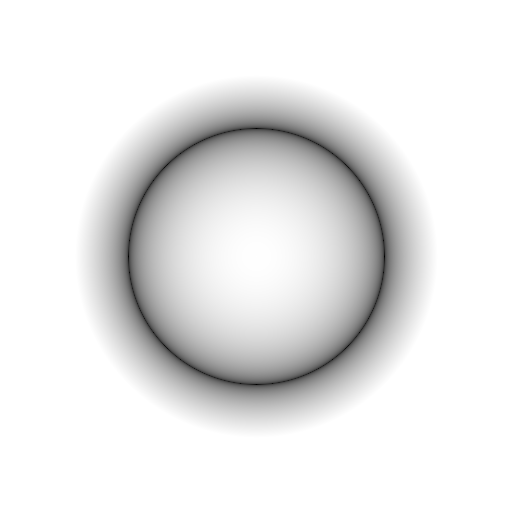
\includegraphics[width=\linewidth]{circle.png}
  \caption{A circle}\label{fig:circle}
\endminipage\hfill
\minipage{0.32\textwidth}
  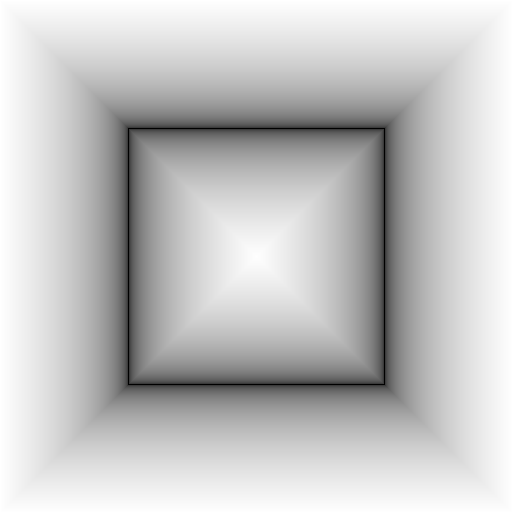
\includegraphics[width=\linewidth]{square.png}
  \caption{A square}\label{fig:square}
\endminipage\hfill
\minipage{0.32\textwidth}%
  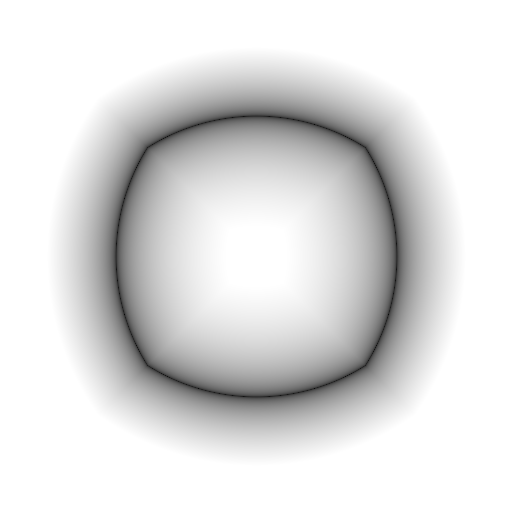
\includegraphics[width=\linewidth]{squircle.png}
  \caption{A squircle}\label{fig:squircle}
\endminipage
\end{figure}
Pixels' color depends on the absolute distance\footnote{gamma corrected and clamped in $[0,1]$} from the surface.
Note that this images can be seen as 2D section of 3D objects done with a yz-aligned plane\footnote{assuming that x grows to the right, y up, and z ``towards" the image} passing through the origin.
The distance equation for the circle is $x^2 + y^2 - 1$, meanwhile for the square it is $max(\abs{x}, \abs{y}) - 1$.
To get a better understanding of the square's SDF we suggest this Quilez's video \cite{iquilez_sdf_box} (and the others on his channel).
% TODO \todo[inline]{If space and time explain here in few lines}
The squircle is the mixing of the square and circle SDFs and its implicit equation is
$ k * (max(\abs{x}, \abs{y}) - 1) + (1-k) * (x^2 + y^2 - 1) $, where $k \in [0,1]$.
This is only one example of the operation we can perform on implicit surfaces.


\subsection{Constructive Solid Geometry}
One of the major benefits we get using SDFs is the easiness with which we can create complex shapes from few primitives, technique known as Constructive Solid Geometry (CSG).
CSG with Boolean operations is largely used in CAD software.
%As said in \cite{hart1996, scratch_sdf, iquilez_sdf}
With DIFs we can simulate:
\begin{itemize}
  \item union with the minimum, because we ``stop" at the first surface that as been found
    $$ min(f_1, f_2) $$
  \item intersection with the maximum, because we ``ignore" the first surface if there's another after
    $$ max(f_1, f_2) $$
  \item subtraction with the maximum between the first surface and the opposite of the second
    $$ max(f_1, -f_2) $$

  \item mixing, creating a shape that is in between of the given two, with interpolation of distances
    $$ k*f_1 + (1-k) * f_2 \;\;\; \text{with $k\in[0,1]$} $$
\end{itemize}
%One interesting operation is blending % TODO?
Here we listed the most common operations, but in theory we can use any mathematical function: sine, cosine, modulo, exponential, etc\dots
All these operations can be arranged in a tree structure, even if the optimal evaluation order may not be always obvious.

%% TODO
%\todo[inline]{
%  Here I can add at least an half-page on blending \\
%  \href{https://www.iquilezles.org/www/articles/smin/smin.htm}{Inigo's article on blending}
%}

Note that the signed distance bound functions are closed by CSG operations so we do not have to handle new cases when we manipulate the resulting shapes.

\begin{figure}[!htb]
\minipage{0.32\textwidth}
  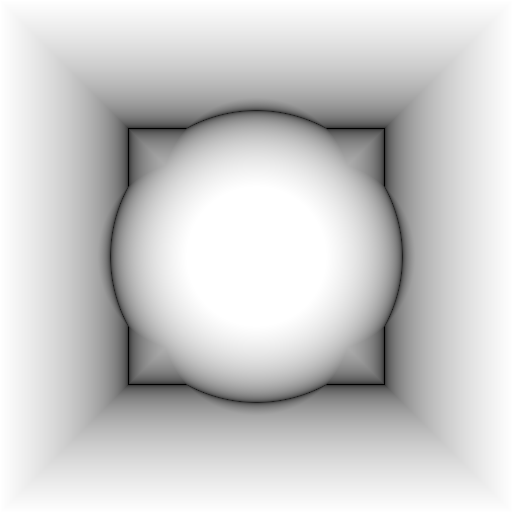
\includegraphics[width=\linewidth]{circle_square_union.png}
  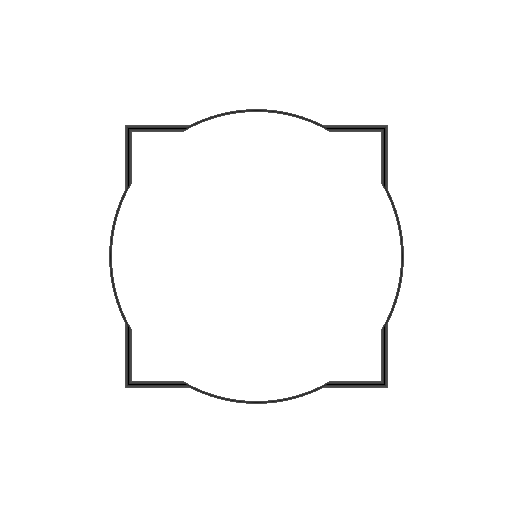
\includegraphics[width=\linewidth]{circle_square_union_c.png}
  \caption{Square-Circle union and its contour}\label{fig:union}
\endminipage\hfill
\minipage{0.32\textwidth}
  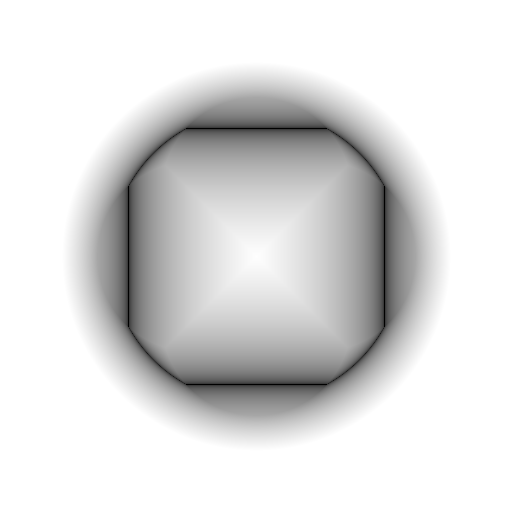
\includegraphics[width=\linewidth]{circle_square_intersection.png}
  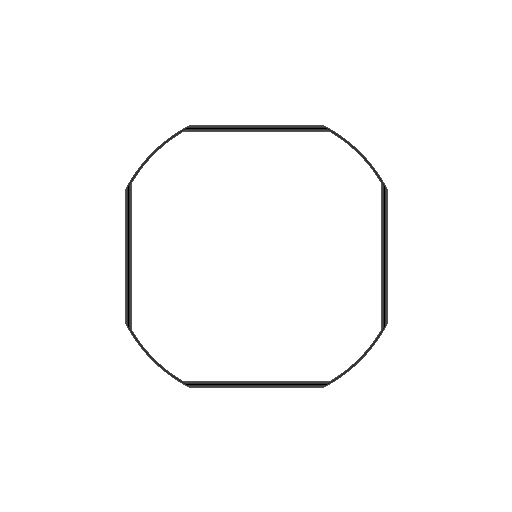
\includegraphics[width=\linewidth]{circle_square_intersection_c.png}
  \caption{Square-Circle intersection and its contour}
  \label{fig:intersection}
\endminipage\hfill
\minipage{0.32\textwidth}%
  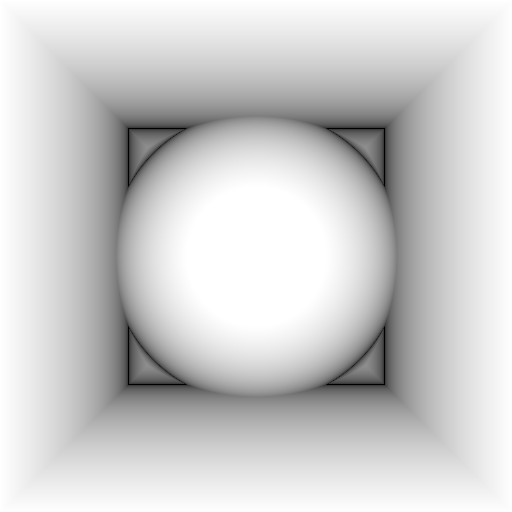
\includegraphics[width=\linewidth]{circle_square_subtraction.png}
  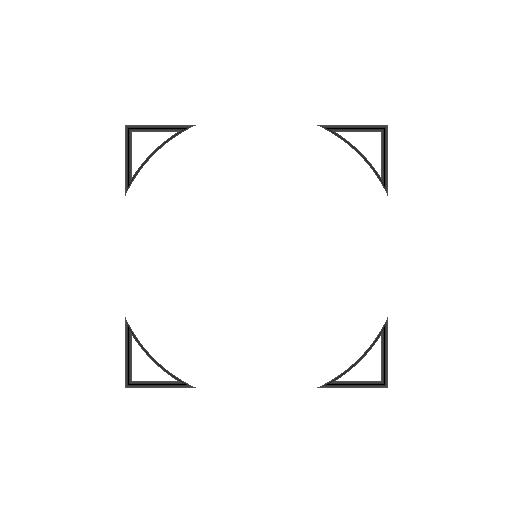
\includegraphics[width=\linewidth]{circle_square_subtraction_c.png}
  \caption{Square-Circle subtraction and its contour}
  \label{fig:subtraction}
\endminipage
\end{figure}
\begin{figure}[!htb]
  \centering
  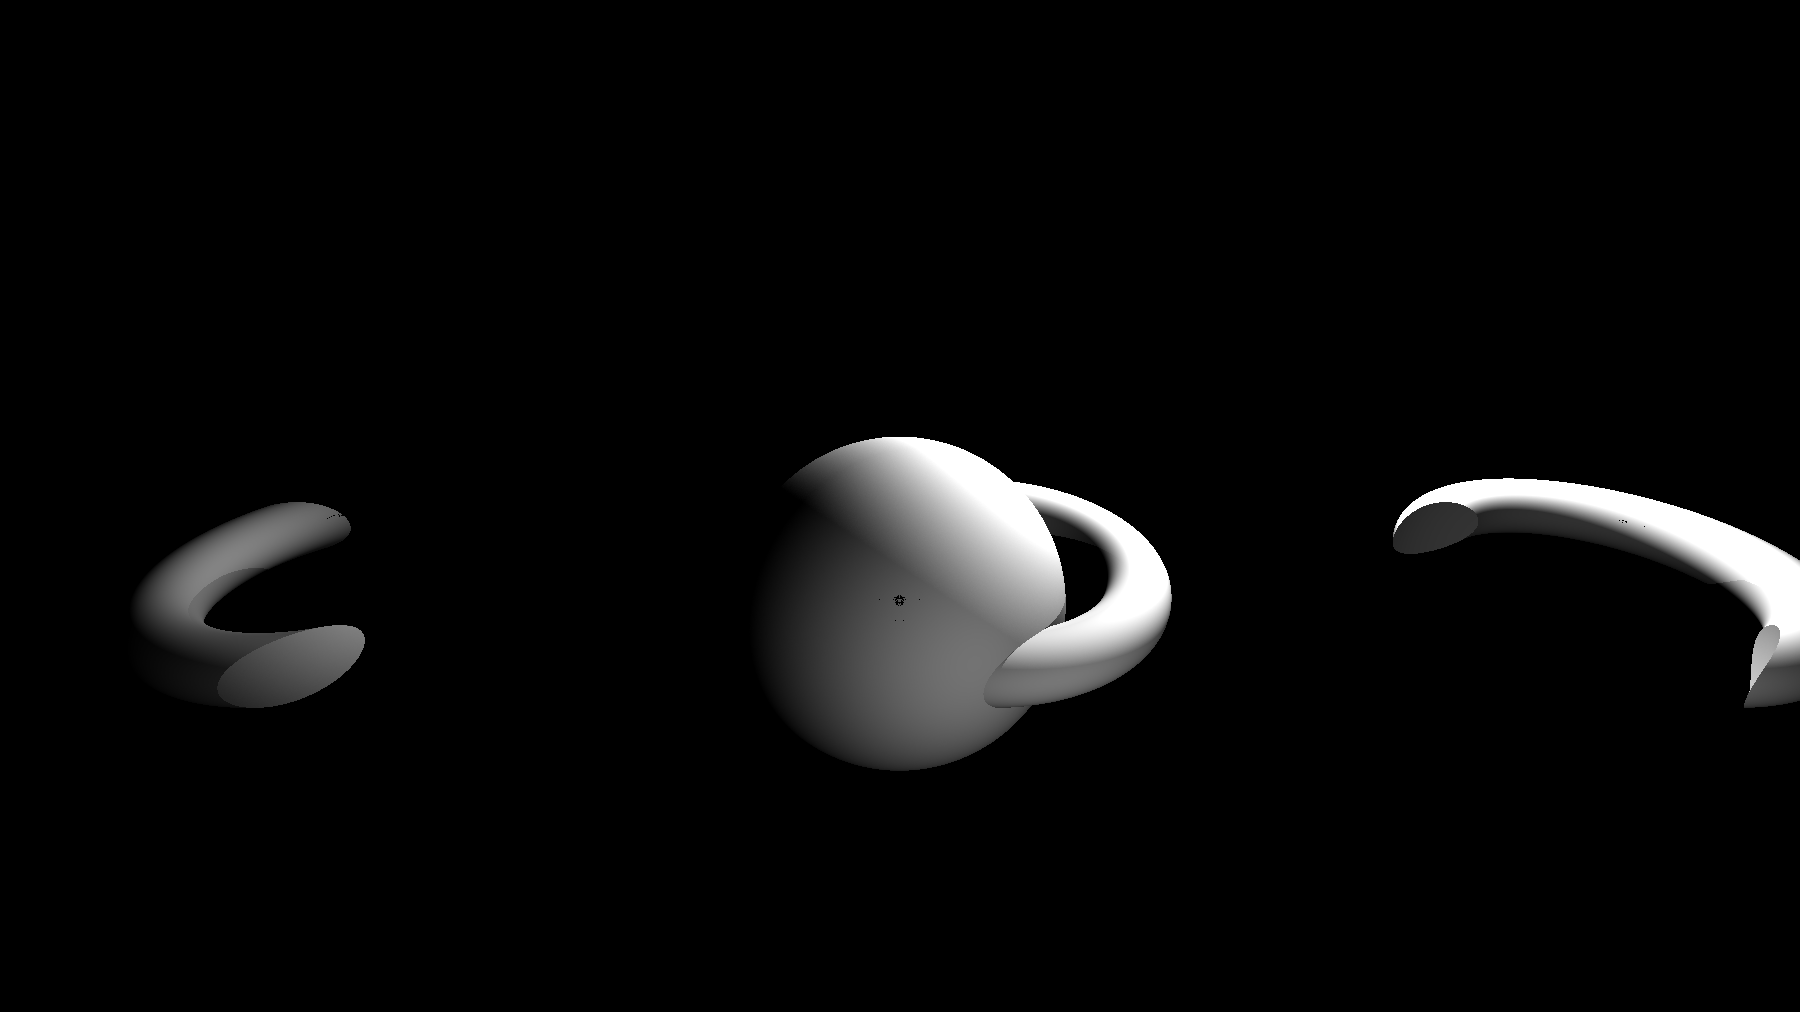
\includegraphics[width=\linewidth]{img_03.png}
  \caption{Left to right:
    intersection, union and subtraction of a sphere and a torus.
    TODO produce better image
  }
  \label{fig:csg}
\end{figure}

